

% Case Study Chapter: Expanded and Enhanced
\subsection*{1. Introduction: Humanizing Threat Modeling}
This chapter brings threat modeling to life through a detailed, humanized case study of the Damn Vulnerable Web Application (DVWA)\cite{owasp}. Rather than simply listing steps, it immerses the reader in the mindset of both attacker and defender, showing how real-world knowledge, technical skill, and strategic thinking converge to protect digital assets. The narrative is designed to deliver deep insight, practical wisdom, and a book-like experience that goes beyond checklists to reveal the true art and science of cybersecurity.

\subsection*{2. Asset Identification and Business Impact}
Every effective security strategy begins with understanding what is at stake. In our case study, the security team starts by cataloging all assets that require protection. These include user credentials (usernames and passwords), session tokens, user data (notes, files, and personal information), the application’s source code, and the backend database\cite{nist800154}. Each asset is evaluated not just for its technical value, but for its business impact—what would happen if it were compromised? This holistic approach ensures that the threat model is grounded in real organizational priorities, not just technical details.

\subsection*{3. Attack Surface Mapping and System Context}
With assets identified, the next step is to map the attack surface—the sum of all points where an attacker can interact with the system\cite{owasp}. The team visualizes the web login form, REST API endpoints, database connections, and the admin panel, considering how each could be targeted. This process is not just technical; it requires creative thinking and empathy for the adversary’s perspective. By walking through the system as an attacker would, defenders uncover hidden risks and design more effective controls. The attack surface map becomes a living document, updated as the system evolves and new threats emerge.
\begin{figure}[H]
	\centering
	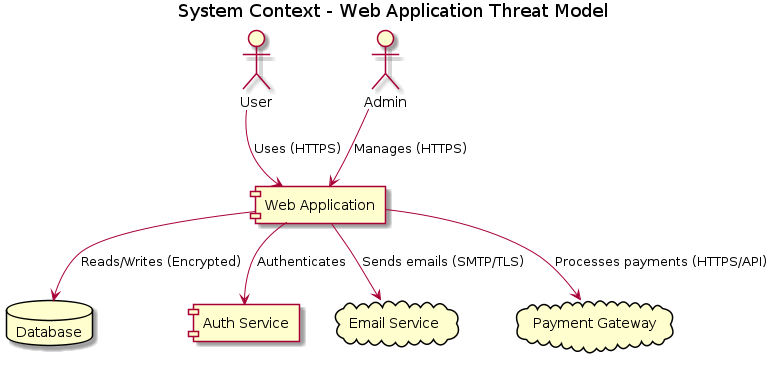
\includegraphics[width=0.7\textwidth]{images/system-context}
	\caption{System Context Diagram for Case Study}
\end{figure}

\subsection*{4. Reconnaissance and Scanning: Attacker’s Perspective}
Reconnaissance is the art of gathering intelligence. The team uses Linux tools to probe the system, uncovering open ports, running services, and technologies in use\cite{shostack2014}. Commands like `nmap` reveal the network’s structure, while `gobuster` and `whatweb` expose hidden directories and software versions. This phase is both technical and psychological: defenders must anticipate the attacker’s curiosity, persistence, and ingenuity. The insights gained here inform every subsequent step, shaping the threat model and guiding defensive strategy.
\begin{verbatim}
# Discover open ports
nmap -sV -T4 -p- 10.0.0.5

# Enumerate web directories
gobuster dir -u http://10.0.0.5 -w /usr/share/wordlists/dirb/common.txt

# Identify technologies
whatweb http://10.0.0.5
\end{verbatim}

\subsection*{5. Vulnerability Scanning and Analysis}
Armed with reconnaissance data, the team turns to vulnerability scanning. Tools like `sqlmap` and `nikto` automate the search for weaknesses, probing for SQL injection, cross-site scripting (XSS), and other common flaws\cite{owasp}. This process is rigorous and methodical, but also creative—defenders must think beyond the obvious, considering how attackers might chain vulnerabilities or exploit subtle misconfigurations. The results are documented, prioritized, and mapped to business risks, ensuring that remediation efforts are both effective and efficient.
\begin{verbatim}
# Scan for SQL injection
sqlmap -u "http://10.0.0.5/login.php" --forms --batch

# Check for XSS
nikto -h http://10.0.0.5
\end{verbatim}

\subsection*{6. Exploitation: Turning Theory into Reality}
The final phase is exploitation—the moment when theory meets reality. Here, the team demonstrates how attackers might leverage identified vulnerabilities to gain unauthorized access or extract sensitive data\cite{uceda2015}. Commands like `sqlmap --dump` show how a simple flaw can lead to catastrophic data loss, while brute-force attacks on weak admin passwords highlight the importance of strong authentication. This section is not just a technical walkthrough; it is a call to action, reminding readers that every vulnerability is a story waiting to be told—and prevented.
\begin{verbatim}
# Exploit SQL injection to dump users
sqlmap -u "http://10.0.0.5/login.php" --dump

# Exploit weak admin password
hydra -l admin -P /usr/share/wordlists/rockyou.txt 10.0.0.5 http-post-form \
"/admin/login.php:username=^USER^&password=^PASS^:F=incorrect"
\end{verbatim}

\subsection*{7. Threat Enumeration (STRIDE/PASTA)}
	extbf{Definition:} Threat enumeration maps discovered vulnerabilities to threat categories\cite{shostack2014,uceda2015}.
\begin{itemize}
	\item Spoofing: Brute-force login, session fixation
	\item Tampering: SQL injection, file upload
	\item Repudiation: Lack of logging
	\item Information Disclosure: Sensitive data in responses
	\item Denial of Service: Flooding login endpoint
	\item Elevation of Privilege: Exploiting admin panel
\end{itemize}

\subsection*{8. Mitigation Strategies and Defensive Wisdom}
	extbf{Definition:} Mitigations are controls that reduce the likelihood or impact of threats\cite{owasp}.
\begin{itemize}
	\item Enforce strong authentication (MFA, password policy)
	\item Use parameterized queries and ORM
	\item Implement audit logging
	\item Encrypt sensitive data in transit and at rest
	\item Rate limit login attempts
	\item Restrict admin panel access
\end{itemize}

\subsection*{9. Academic Perspective and Further Reading}
For deeper understanding, refer to:
\begin{itemize}
	\item Tony UcedaVélez and Marco M. Morana, "Risk Centric Threat Modeling" (Wiley, 2015)
	\item Adam Shostack, "Threat Modeling: Designing for Security" (Wiley, 2014)
	\item NIST SP 800-154: Guide to Data-Centric System Threat Modeling
	\item OWASP Threat Modeling Cheat Sheet
\end{itemize}
